The forensics team started by investigating the physical exterior of the machine, looking for clues which may alude to its function. This section discusses their methodologies and findings in detail.


\subsection{Technical number enquires}

\begin{figure}[h]
	\centering
	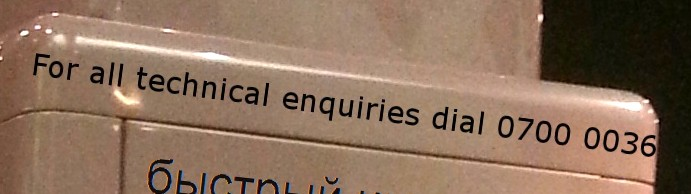
\includegraphics[width=0.8\columnwidth]{img/phone-enquiries.jpg}
	\caption{Technical enquiries phone number}
	\label{fig:technical-enquiries}
\end{figure}

The message in Figure~\ref{fig:technical-enquiries} was prominantly displayed near the top of the machine. A look up of historical phone directory records traced the number back to the \emph{ORSA Journal on Computing}. 
A follow up visit was made to their customer services branch (Figure~\ref{fig:orsa-map}):

\begin{quote}
5521 Research Park Drive \\
Suite 200 \\
Catonsville, Maryland 21228-4664 \\
USA
\end{quote}

\begin{figure}[h]
	\centering
	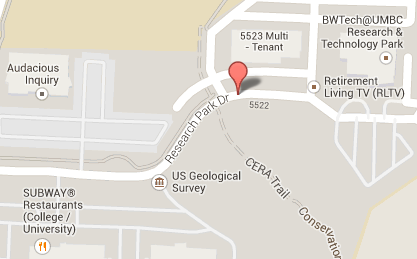
\includegraphics[width=0.95\columnwidth]{img/orsa.png}
	\caption{ORSA Journal on Computing customer services branch. Brunch was purchased from \protect 
\includegraphics[height=0.98em,keepaspectratio]{img/subway.png}.}
	\label{fig:orsa-map}
\end{figure}

The team was then able to retrieve an excerpt\footnote{An online version was independantly found at \url{http://www.columbia.edu/~ww2040/Fall03/LaplaceInversionJoC95.pdf}} of a document \emph{Numerical Inversion of Laplace Transforms of Probability Distributions}.



\subsection{Cyrillic script}
Some Cyrillic script was found on the machine, believed by our Business and Strategy experts to be used for marketing the machine in the Russian market.

An image of the script was analyzed and translated electronically (Figure~\ref{fig:cyrillic-script}), yielding the rough English translation of \emph{Fast inverter integrated functions}.

\begin{figure}[h]
	\centering
	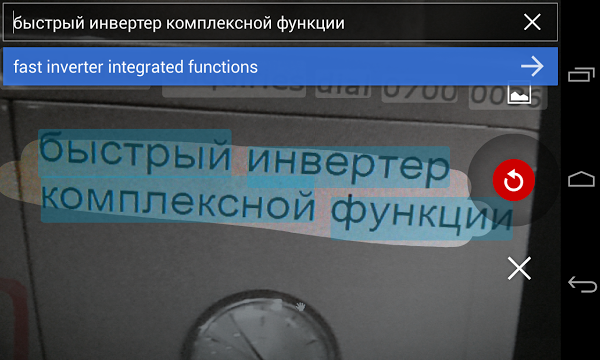
\includegraphics[width=0.9\columnwidth]{img/cyrillic-script.png}
	\caption{Cyrillic script found on the machine, along with the analysis results.}
	\label{fig:cyrillic-script}
\end{figure}

It is speculated that this marketing campaign was highly unsuccessful, as the marketing text consisted merely of a catchy phrase with no detailed description of operation \footnote{Catchy marketing phrases are clearly an inferior marketing technique, and would never work --- c.f. ``Just do it'' and ``I'm lovin' it'' for examples of such unsuccessful campaigns.}. Additionally, the provided help instructions were provided in a crude mixture of English and French, probably unhelpful for the Russian operators.




\subsection{Geographic coordinates}
The geographic coordinates $2.3328700E \; 48.8074800N$ were found inscribed on the machine. However, due to a lack of 3G signal in the basement, the geographic team were unable to access the internet and hence encountered difficulties in determining the whereabouts of the coordinates inscripted on the machine. The issue was promptly escalated to the CTO, who commissioned the purchase of two horses from a local supermarket. \footnote{Despite the falling price of petrol, it remains beyond our budget. As a plus, horses are also free to park.}

The location was found to be near the Laplace train station in France (Figure~\ref{fig:laplace-horses}). Realising the mismatch in units due to the ``inverse function'' applied to the coordinates, the agents determined that the devious scheme was intended to be a very subtle hint that the machine may be performing an inverse Laplace transform. In order to cut costs, the horses were auctioned off at the nearby \emph{Square du Serment de Koufra} for a profit of \EUR{7.89}. This was sufficient to purchase baguettes for lunch.

\begin{figure}[h]
	\centering
	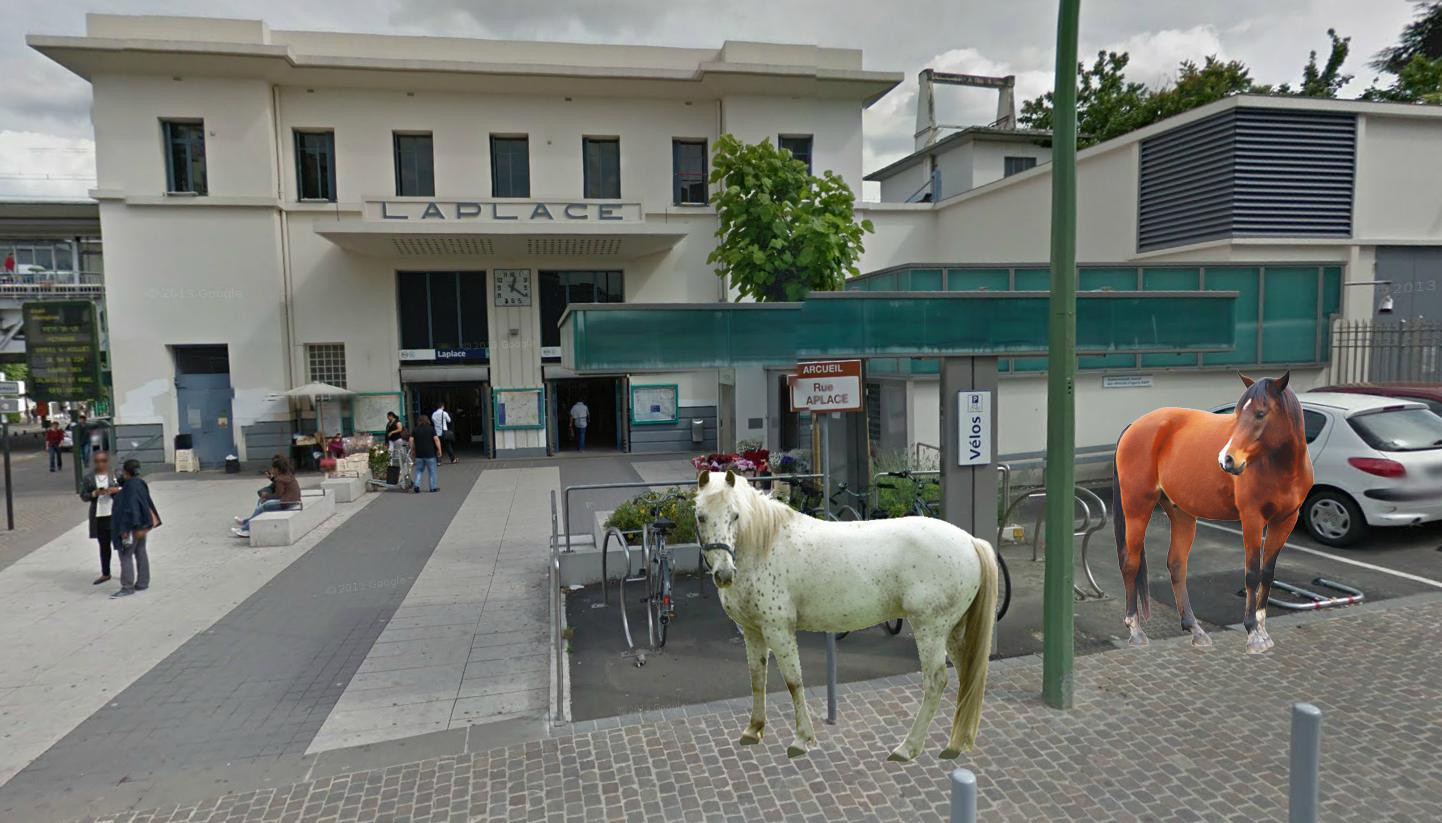
\includegraphics[width=0.95\columnwidth]{img/laplace-horses.jpg}
	\caption{Straight ahead: the main enterance of the Laplace train station. Right: the parked horses.}
	\label{fig:laplace-horses}
\end{figure}



\subsection{Portrait}
% Google colors
\definecolor{google-blue}{HTML}{0266C8}
\definecolor{google-red}{HTML}{F90101}
\definecolor{google-yellow}{HTML}{F2B50F}
\definecolor{google-green}{HTML}{00933B}
\newcommand{\google}{\textcolor{google-blue}{G}\textcolor{google-red}{o}\textcolor{google-yellow}{o}\textcolor{google-blue}{g}\textcolor{google-green}{l}\textcolor{google-red}{e}}

A grayscale portrait was located on the central axis of the machine (Figure~\ref{fig:euler}). As the portrait's CMYK band was much too narrow for our forensic experts' eyes, an image was instead captured and sent to the \textcolor{google-blue}{G}l\textcolor{google-red}{O}bal cl\textcolor{google-yellow}{O}ud-based \textcolor{google-blue}{G}enealogy \textcolor{google-green}{L}ocator \textcolor{google-red}{E}-service (\google). The subject was identified as Leonhard Euler,``a pioneering Swiss mathematician and physicist'' (according to an omni-reliable, omni-malleable source \footnote{Wikipedia, the free encyclopedia}). This may hint that the machine employs Euler's methods for its computation.

\begin{figure}[h]
	\centering
	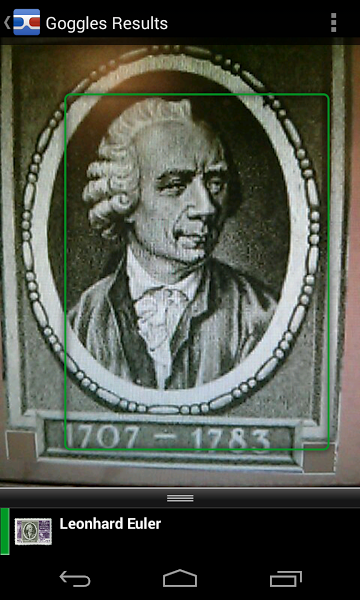
\includegraphics[width=0.8\columnwidth]{img/euler.png}
	\caption{The result of the analysis on the portrait reveals the subject to be Leonhard Euler.}
	\label{fig:euler}
\end{figure}



\subsection{Wall clock and CRT Display}

The machine panel has two seemingly, and deceivingly, unrelated components.

\begin{figure}[h]
	\centering
	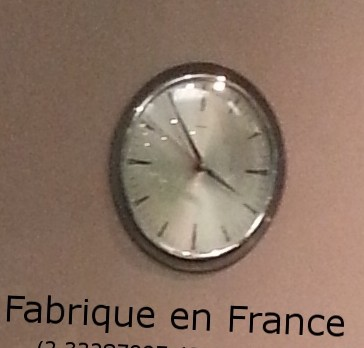
\includegraphics[width=0.8\columnwidth]{img/clock.jpg}
	\caption{The wallclock located on the main panel of the machine}
	\label{fig:clock}
\end{figure}

Firstly we have the wall clock (Figure ~\ref{fig:clock}), indicating the current time (as clocks do) to be $3:55$, or more likely $15:55$ given the sunlight in the background. Since Nukehavistan is located around $31N$ latitude (Figure~\ref{fig:map}), we are not dealing with a case of midnight sun\footnote{\url{http://en.wikipedia.org/wiki/Midnight_sun}}.

\begin{figure}
	\centering
	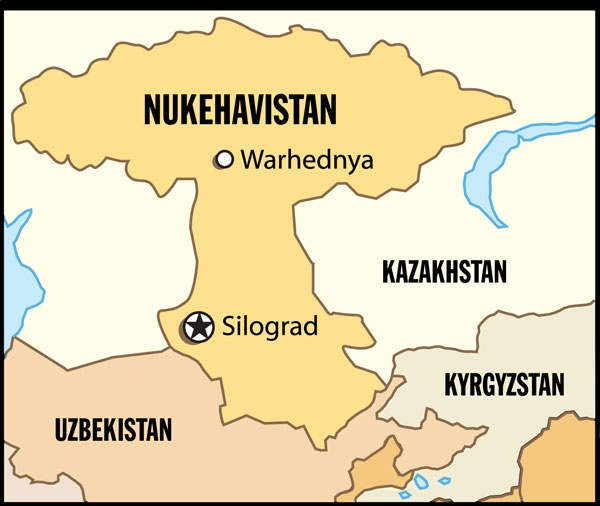
\includegraphics[width=0.8\columnwidth]{img/nukehavistan.jpg}
	\caption[A map of the Republic of Nukehavistan]{A map of the Republic of Nukehavistan \protect \footnotemark}
	\label{fig:map}
\end{figure}
\footnotetext{Image courtesy of The Onion \\ \url{http://www.theonion.com/articles/us-intelligence-nukehavistan-may-have-nuclear-weap,1373/}}


Secondly we have the CRT display (Figure~\ref{fig:crt}), which shows a graph of some function $f(t)$ over time. The graph has a positive peaks at $t = 3$ and a negative peak at $t = 11$. 

\begin{figure}[h]
	\centering
	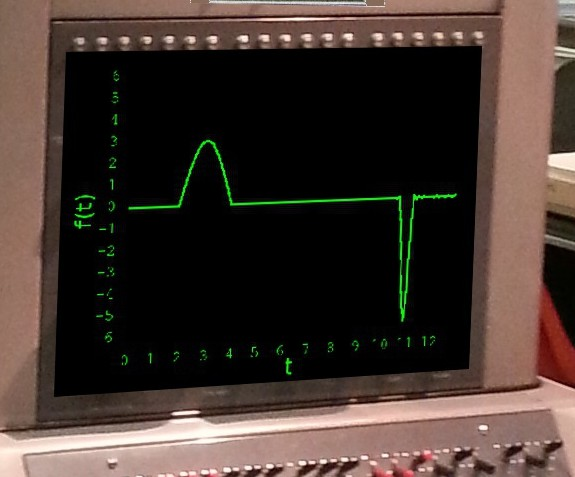
\includegraphics[width=0.8\columnwidth]{img/crt.jpg}
	\caption{The CRT display showing a live graph in neon-ish green.}
	\label{fig:crt}
\end{figure}

After copious degrees of analysis, it was determined that the peaks in the graph are actually mirroring the hands of the clock, the positive peak representing the position of the hour hand (rounded down to the current hour), and the negative peak representing the position of the minute hand (rounded down to the nearest multiple of five). The fact that the $t$ axis runs from $0$ to $12$ further supports this argument. Thus the graph in the image points at $3$ (as is the current hour) and $11$, translating to minutes $55-59$ (as is the current minute).

The circuit board is therefore used to plot a curve representing the current (12-hour) time (Figure~\ref{fig:essentially}).

\begin{figure}[h]
	\centering
	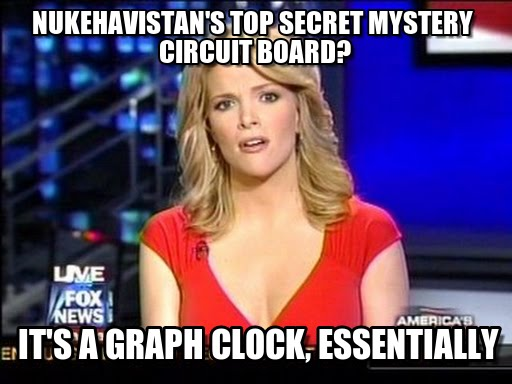
\includegraphics[width=0.8\columnwidth]{img/essentially.jpg}
	\caption{Fox news anchor Megyn Kelly commenting on the discovery.}
	\label{fig:essentially}
\end{figure}
